\section{前期准备}
\subsection{贡嘎环线}

\begin{figure}[htbp]
  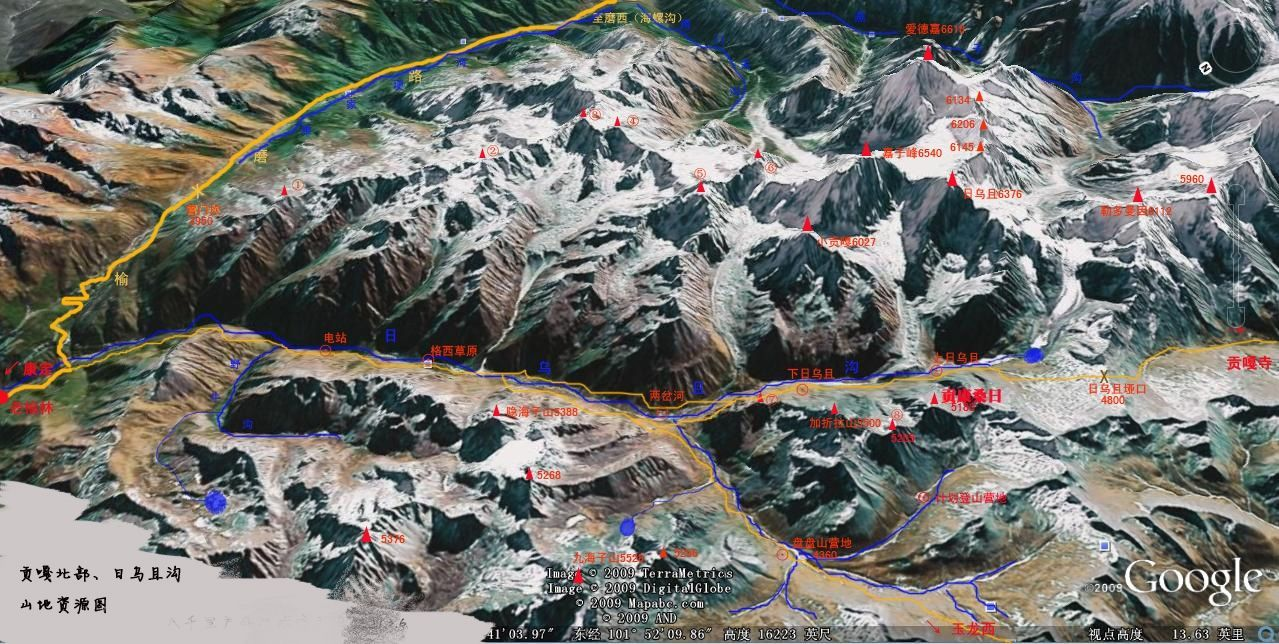
\includegraphics[width=1.0\textwidth]{shandi.jpg}
\end{figure}
\begin{figure}[htbp]
  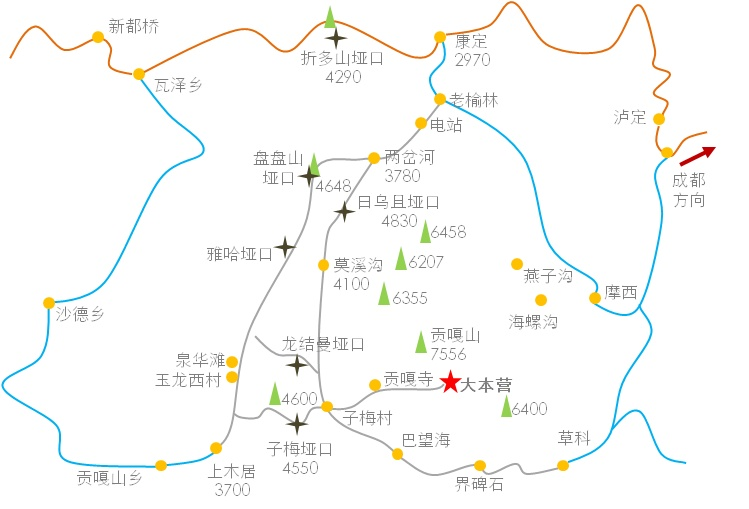
\includegraphics[width=1.0\textwidth]{map1.jpg}
\end{figure}
\begin{figure}[htbp]
  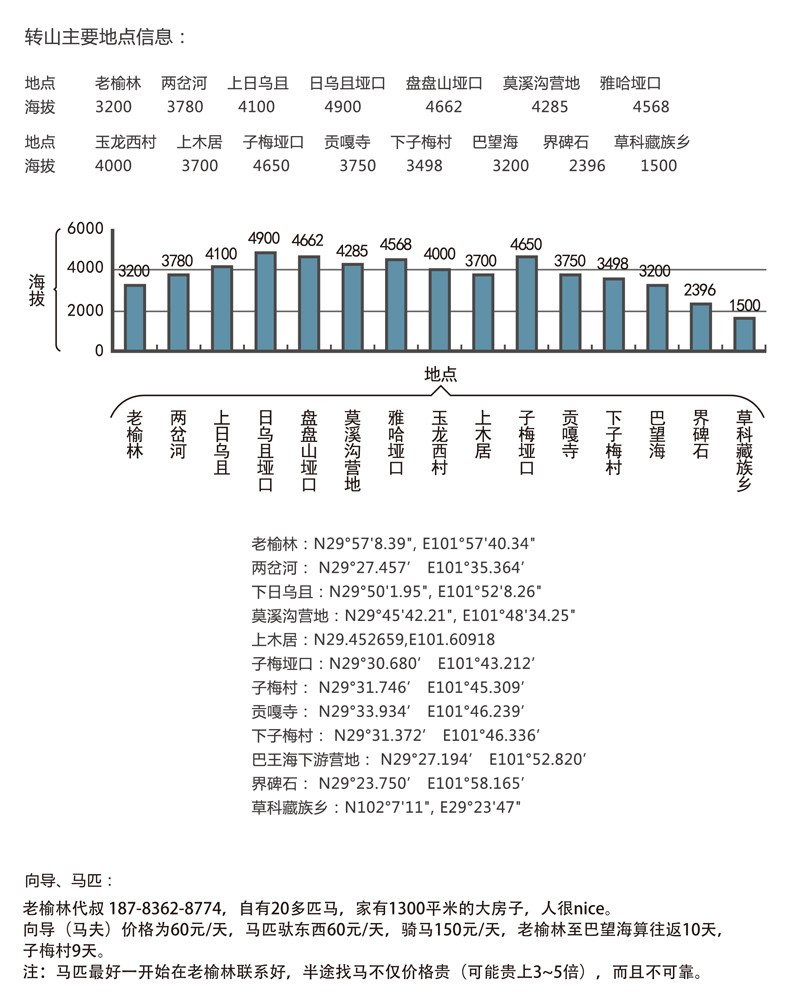
\includegraphics[width=1.0\textwidth]{inf.jpg}
\end{figure}

\subsection{装备购置}
\subsubsection{服装装备}
\begin{itemize}
  \item 冲锋衣(防风,防水,透气,耐磨)
  \item 抓绒衣 (含windstopper,防风保暖)
  \item 排汗内衣(保持身体干燥,防止失温)
  \item 羽绒衣裤,雨衣
  \item 个人衣物(一次性内裤,等)
  \item 徒步鞋, 溯溪鞋,登山鞋
  \item 排汗袜 (最好是coolmax面料,配合gore-tex穿,可排脚汗,防冻伤和起水泡)
  \item 遮阳帽,抓绒帽,厚手套,雪镜或墨镜,头巾
\end{itemize}
\subsubsection{辅助装备}
\begin{itemize}
  \item 保温水壶
  \item 头灯,手电
  \item 登山杖
  \item 护膝
  \item 雪套?(在雪地和泥泞的公路很管用?)
  \item 登山包(建议60升或以上),冲锋包?(小包,背负路餐及其他用品),可能要驮包?(用以马托运)
  \item 防水袋
  \item 纸质地图,指南针,军刀,求生哨,对讲机
  \item 打火机
\end{itemize}
\subsubsection{露营装备}
\begin{itemize}
  \item 睡袋(极限温标至少-15度以下)
  \item 帐篷(四季帐或高山帐),帐灯?
  \item 帐篷地席(保护你的帐篷底面,免受磨损)
  \item 防潮垫(泡沫垫或充气垫)
  \item 铝膜地席(选择性带)
  \item 炉头,气罐,套锅(用于烧水煮茶),高压锅?
\end{itemize}
\subsubsection{医疗用品}
\begin{itemize}
  \item 处方药:乙酰唑胺、综合维他命、硝苯地平和低塞米松--处方药,有副作用,需在药师指导下依照个人情况服用\\
        乙酰唑胺可增加肺通气量,提高血氧饱和度和睡眠质量。乙酰唑胺可减轻高原病症状,有降低高原病发病率的倾向。地塞米松属于短期防治急性高原反应的药物。地塞米松能预防急性高原病,可以预防高原肺水肿的发生。\\
        非处方药:阿司匹林、芬必得--镇痛药,对缓解高反引起的头痛有较好的疗效,可以相应地改善身处高海拔营地时的睡眠质量;红景天可以增加血液流动性,改善缺氧,改善高反状况。\\
        救生毯--可以隔绝皮肤与寒冷空气的接触,其含有的金属成分可以反射身体的热辐射,最大限度锁住身体热量的流失,避免失温加剧。
\end{itemize}
\subsubsection{生活用品}
\begin{itemize}
  \item 餐具
  \item 路餐
  \item 贴身
\end{itemize}
\subsubsection{其他}
\begin{itemize}
  \item 移动电源,数据线
  \item 学生证,身份证
  \item 真空袋,环保袋,卫生纸
  \item 打火石,镊子
  \item 军刀
\end{itemize}

\subsection{相关网址}
\begin{itemize}
  \item 如何制作手机离线地图?\\
   \url{http://www.8264.com/wenzhang/5510614.html}
  \item 徒步也有套路:7种不同路面,7种徒步技巧\\
    \url{http://www.8264.com/viewnews-128290-page-1.html}
\end{itemize}
\subsection{训练计划}